\chapterauthor{Jeferson J. Lima}{Departamento de Informática (DAINF) \\Universidade Tecnológica Federal do Paraná (UTFPR)}
\chapter{Conceitos Básicos}

 
\section{Introdução}\label{intro::cap3}

As técnicas de localização aplicadas na robótica móvel fornecem uma estimativa da posição do um robô em relação as coordenas iniciais, sendo este um mapa ou qualquer outro modelo de referência.

A percepção destas coordenadas se dá através de uma série de sensores que fornecem um estimativa da localização o robô durante determinado movimento. Esse predição do estado é executada interativamente em intervalos de tempo, determinados pela frequência de operação dos sensores. 

Assim, a crença do estado atual pode ser encontrada e os dados adqueridos dos sensores, podem então, ser traduzidos em mapas a qual o mesmo robô ou outros robôs podem recorrer para melhorar a crença da posição atual.

\section{Filtro de Bayes}

O Filtro de Bayes é o algoritmo em diversas técnicas de auto-localização onde pretende-se resolver a manutenção da crença da posição de um robô, com base nos seus estados. O algoritmo calcula a densidade de probabilidade que se traduz na crença do robô a partir de dados dos sensores e o modelo de controle do robô  \cite{thrun2006probalistic}. A solução deste problema de auto-localização, utilizando-se da inferência bayesiana, está em encontrar o valor esperado da posição em cada instante de tempo, conforme a \eq{eq:bayes1}.

\begin{equation}
    \label{eq:bayes1}
    \hat X_t = E\left[X_t| z_t, u_t\right] = \displaystyle \int\limits_x x P(X_t = x| z_t, u_t)\text{d}x
\end{equation}

Para este problema, o algoritmo do Filtro de Bayes apresenta-se como uma forma recursiva, \eq{eq:bayes2}, onde $\text{Bel}(x_t)$ representa a função densidade da crença no tempo $t$ e $\text{Bel}(x_{t-1})$ a função no intervalo de tempo anterior. A relação entre o intervalo de tempo das interações do filtro, será definida, conforme citado acima pela velocidade de operação dos sensores envolvidos, aqui apresentados como $z_t$. O termo $u_t$ representa a variável de ação do modelo ou variável de controle.


\begin{equation}
    \label{eq:bayes2}
    \text{\text{Bel}}(x_t) = \eta P(z_t| x_t) \int P(x_t| u_t, x_{t-1}) \text{Bel}(x_{t-1})\text{d}x_{t-1}
\end{equation}


A esta primeira fase do algoritmo, a qual calcula a distribuição em relação a crença dos estados $x_{t-1}$ e $u_t$, é chamada de predição e o resultado da função crença é dada por $\overline{\text{Bel}}(x_t)$.

Na segunda fase, chamada aqui de correção, a crença $\overline{\text{Bel}}(x_t)$ é multiplicada pela probabilidade dos estados observados em relação ao sensores $z_t$.

\begin{algorithm}[H]
    \caption{Filtro de Bayes}
    \begin{algorithmic}[1]
    \Procedure{predição}{$\text{Bel}(x_{t-1}), u_t$}
        \State $\overline{\text{Bel}}= \displaystyle\int P(x_t| u_t, x_{t-1})\text{Bel}(x_{t-1})\text{d}x_t$
    \EndProcedure
    \Procedure{Correção}{$\overline{\text{Bel}}(x_{t}), z_t$}
        \State ${\text{Bel}}= \displaystyle\textcolor{white}{\int}  \eta P(z_t| x_{t})\overline{\text{Bel}}(x_{t})$
    \EndProcedure
    \State Normatiza $\eta \displaystyle\int \text{Bel}(x_t)\text{d}x_t = 1$
    \State \textbf{Retorne} $\text{Bel}(x_t)$

    \end{algorithmic}
\end{algorithm}

O algoritmo finaliza com a crença normatizada e a estimativa da posição do robô é calculada. O algoritmo do Filtro de Bayes apresentado aqui é aplicável apenas a uma classe de problemas simples, no entanto serve de base para implementações mais complexas onde a cinemática e dinâmica do sistemas são consideradas, como no exemplo do Filtro de Kalman a ser apresentado abaixo.

\section{Filtro de Kalman}

O Filtro de Kalman é provavelmente a implementação mais aplicada com base no Filtro de Bayes. Proposto por Rudolph Emil Kalman, em 1950 como técnica para filtragem e predição de sistemas lineares. O Filtro proposto por Kalman resolve o problema de observação dos sensores externos do robô, considerando inerentes a leitura dos sensores. \cite{thrun2006probalistic,romero2014robotica}.

A garantia da densidade de probabilidade, apresentada em \eq{eq:bayes2}, é dada por uma aproximação do método apresentado anteriormente. Nesta aproximação o modelo de movimento do robô e o modelo do observador, com base nos sensores, é representado por densidades gaussianas multivariáveis.

A função de densidade gaussiana $P(X = x)$, sendo um $X$ um vetor, pode ser expressa na seguinte forma ${P(X = x) \sim N(\mu, \sigma^2)}$, onde $\mu$ representa a média e $\sigma^2$ a variância da distribuição, conforme a  \eq{eq:gauss1}.

\begin{equation}
    \label{eq:gauss1}
    P(X = x) = \dfrac{1}{\sqrt{2\pi\sigma^2}}\cdot 
    \exp\left\{-\frac{(x-\mu)^2}{2\sigma^2}\right\}
\end{equation}

A Figura \fig{fig::gauss1} apresenta três funções de densidade gaussiana, com os valores respectivamente para $\mu_i = \{0,0,-2\}$ e $\sigma^2_i = \{1,2,1\}$.


\begin{figure}[!ht]
    \centering
    \begin{tikzpicture}[
    declare function={
      normalpdf(\x,\mu,\sigma)=
      (2*3.1415*\sigma^2)^(-0.5)*exp(-(\x-\mu)^2/(2*\sigma^2));
    },
    hplot/.style={ycomb, mark=o, dashed}, ,scale=0.8]
  
    \begin{axis}[
      width=12cm, height=6cm,
      samples=50,
      xlabel=$x$, ylabel=$p(x)$,
      xlabel style={at={(1,0)}, anchor=north west},
      ylabel style={rotate=-90, at={(0,1)}, anchor=south east},
      legend style={draw=none, fill=none},
      domain=-6:9,
      legend cell align=left,
      xmin=-7, xmax=11]
  
      \addplot [smooth, thick] {normalpdf(x,0,1)}
      node[pos=0.47, pin={right:$\mu=0,\sigma^2=1$}] {};
      \addplot [smooth, blue] {normalpdf(x,0,2)}
      node[pos=0.6, pin={45:$\mu=0,\sigma^2=2$}] {};
      \addplot [smooth, red] {normalpdf(x,-2,1)}
      node[pos=0.25, pin={[text centered, text width=8ex]
        200:$\mu=-1$, $\sigma^2=1$}] {};
  
      \addplot [hplot, samples at={0}] {normalpdf(x,0,1)};
      \addplot [hplot, samples at={0}, blue] {normalpdf(x,0,2)};
      \addplot [hplot, samples at={-2}, red] {normalpdf(x,-2,1)};
  
      \node[anchor=north east] at (axis description cs: 0.975,  0.95)
      {$p(x) = \dfrac{1}{\sqrt{2\pi\sigma^2}}\cdot 
        \exp\left\{-\frac{(x-\mu)^2}{2\sigma^2}\right\}$};
  
    \end{axis}
  \end{tikzpicture}
    \caption{Representação de três funções de Distribuição Normal}
    \label{fig::gauss1}
\end{figure}

Um dos requisitos para aplicação do Filtro de Kalman é que o modelo determinístico de observação se haja linear para que haja uma correta aproximação com a densidade de probabilidade, conforme é mostrado na  \eq{eq::linear1d}.


\begin{equation}
    \label{eq::linear1d}
    \left.
    \begin{aligned}
            X & \sim N\left(\mu, \sigma^2\right)\\
            Y & = aX + b\\
    \end{aligned} \right\}
    \quad \Rightarrow \quad Y \sim N\left(a\mu+b\right)
\end{equation}

Os coeficientes $a$ e $b$ são coeficientes lineares do modelo. A \eq{eq::linear1d} possui apenas um estado, no entanto sistemas complexos são tipicamente representados diversos estados e diversos sensores.
Sistemas robóticos possuem vários estados, sendo assim a densidade de probabilidade ${P(\mathbf{x}) \sim N(\boldsymbol{\mu}, \textstyle\sum)}$ é formada por uma  multivariável, onde $\boldsymbol{\mu}$ representa o vetor das médias e ${\textstyle\sum}$ a matriz de covariância, conforme pode ser visto na  \eq{eq::linearNd}.

\begin{equation}
    \label{eq::linearNd}
    P(\mathbf{x}) =\frac{1}{\sqrt{(2\pi)^{d}|\sum|}}\exp\left\{-\frac{1}{2} (\mathbf{x}-\boldsymbol\mu)^T\textstyle\sum{}^{-1}(\mathbf{x}-\boldsymbol\mu)\right\}
\end{equation}

Desta forma, a figura \fig{fig::gauss2} apresenta a distribuição normal para um sistema bivariável.


\begin{figure}[!ht]
    \centering
    \resizebox{0.6\textwidth}{!}{
\pgfplotsset{%
  colormap={whitered}{color(0cm)=(white);
  color(1cm)=(orange!75!red)}
}
\begin{tikzpicture}[
  declare function = {mu1=1;},
  declare function = {mu2=2;},
  declare function = {sigma1=0.5;},
  declare function = {sigma2=1;},
  declare function = {normal(\m,\s)=1/(2*\s*sqrt(pi))*exp(-(x-\m)^2/(2*\s^2));},
  declare function = {bivar(\ma,\sa,\mb,\sb)=
    1/(2*pi*\sa*\sb) * exp(-((x-\ma)^2/\sa^2 + (y-\mb)^2/\sb^2))/2;},scale=0.6]
  \begin{axis}[
    colormap name  = whitered,
    width          = 15cm,
    view           = {45}{65},
    enlargelimits  = false,
    grid           = major,
    domain         = -1:4,
    y domain       = -1:4,
    samples        = 26,
    xlabel         = $x_1$,
    ylabel         = $x_2$,
    zlabel         = {$P$},
    colorbar,
    colorbar style = {
      at     = {(1,0)},
      anchor = south west,
      height = 0.25*\pgfkeysvalueof{/pgfplots/parent axis height},
      title  = {$P(x_1,x_2)$}
    }
  ]
    \addplot3 [surf] {bivar(mu1,sigma1,mu2,sigma2)};
    \addplot3 [domain=-1:4,samples=31, samples y=0, thick, smooth]
      (x,4,{normal(mu1,sigma1)});
    \addplot3 [domain=-1:4,samples=31, samples y=0, thick, smooth]
      (-1,x,{normal(mu2,sigma2)});

    \draw [black!50] (axis cs:-1,0,0) -- (axis cs:4,0,0);
    \draw [black!50] (axis cs:0,-1,0) -- (axis cs:0,4,0);

    \node at (axis cs:-1,1,0.18) [pin=165:$P(x_1)$] {};
    \node at (axis cs:1.5,4,0.32) [pin=-15:$P(x_2)$] {};
  \end{axis}
\end{tikzpicture}}
    \caption{Distribuição Normal Bivariável}
    \label{fig::gauss2}
\end{figure}

Desta forma, a densidade de probabilidade, conforme é mostrado na  abaixo:

\begin{equation}
    \left.
    \begin{aligned}
            X & \sim N\left(\boldsymbol\mu, \textstyle\sum\right)\\
            Y & = {A}_tX + {B_t}\\
    \end{aligned} \right\}
    \quad \Rightarrow \quad Y \sim N\left( {A_t}\boldsymbol\mu+B_t, {A_t}\textstyle\sum {A_t}^T \right)
\end{equation}

Para o caso multivariável, ${A_t}$ e ${B_t}$ são matrizes $n \times n$ e $n \times l$, respectivamente, sendo $n$ o número de estados e $l$ o número de variáveis de controle.

Definida a funções de densidade de probabilidade para um sistema multivariável, tem-se agora que definir o modelo do sistema.
No modelo estocástico do sistema do robô, as incertezas serão acrescentadas, conforme visto pela  \eq{eq::mdinamic}.

    \begin{equation} 
        \label{eq::mdinamic}
        \begin{aligned}
            x_t &= {A}_t x_{t-1} + {B}_t u_t +  w_t\\ 
        z_t &= {C}_t x_t + v_t
        \end{aligned}
        \end{equation}

    Sendo: 

    \begin{itemize}
        \item[-] ${A}_t$ Matriz $(n \times n)$ que descreve os estados do modelo.
        \item[-] ${B}_t$ Matriz $(n \times l)$ que descreve os estados do controle.
        \item[-] ${C}_t$ Matrix $(k\times n)$ sendo os estados de $x_t$.
        \item[-] $w_t$ Variável aleatória do processo com distribuição normal e covariância ${Q}$.
        \item[-] $v_t$ Rúido aleatório com distribuição normal, covariância de ${R}$.
    \end{itemize}

Para solução numérica algumas considerações precisam ser aplicadas a  \eq{eq:bayes2}, conforme mostra a tabela abaixo:

\begin{equation*}
    \begin{array}{ll}
        Bel(x_t) & \Rightarrow\textcolor{white}{\displaystyle\int} P(x_t| u_1, z_1,  \cdots, z_t) \\
        Bayes & \Rightarrow\textcolor{white}{\displaystyle\int} \eta P(z_t|x_t,  u_1, z_1,  \cdots,  u_t)P(x_t, u_1, z_1, \cdots, u_t) \\
        Markov & \Rightarrow\textcolor{white}{\displaystyle\int} \eta P(z_t|x_t)P(x_t, u_1, z_1, \cdots, u_t) \\
        Prob. Total & \Rightarrow\textcolor{white}{\displaystyle\int} \eta P(z_t|x_t)\displaystyle\int P(x_t| u_1, z_1, \cdots, u_t,x_{t-1})P(x_{t-1}| u_1, z_1, \cdots, u_t)\text{d}x_{t-1}\\
        Markov & \Rightarrow\textcolor{white}{\displaystyle\int} \eta P(z_t|x_t) \displaystyle\int P(x_t| u_t,x_{t-1})P(x_{t-1}| u_1, z_1, \cdots, u_t)\text{d}x_{t-1} \\
        Markov & \Rightarrow\textcolor{white}{\displaystyle\int} \eta P(z_t|x_t) \displaystyle\int P(x_t| u_t,x_{t-1}){P(x_{t-1}| u_1, z_1, \cdots, z_{t-1}}){\text{d}x_{t-1}} \\
    \end{array}   
\end{equation*}
Temos então:

\begin{equation*}
    \textcolor{blue}{\text{Bel}(x_t)} =\eta \textcolor{purple}{P(z_t|x_t)}\displaystyle\int \textcolor{red}{P(x_t| u_t,x_{t-1})}\textcolor{gray}{\text{Bel}(x_{t-1})}\text{d}x_{t-1}
\end{equation*}


Desta forma, o Filtro de Kalman fornece a densidade de probabilidade para posição do robô, por exemplo. De uma forma simplificada, a solução de Kalman é demonstrada pelo figura \fig{fig::kalm1}.

A figura \fig{fig::kalm1} demonstra graficamente a equação acima, com relação função de densidade de probabilidade em relação aos estados do robô.
    
\begin{figure}[!ht]
    \centering
        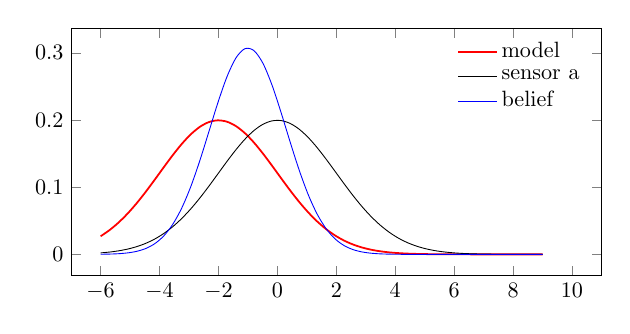
\begin{tikzpicture}[
      declare function={
        normalpdf(\x,\mu,\sigma)=
        (2*3.1415*\sigma^2)^(-0.5)*exp(-(\x-\mu)^2/(2*\sigma^2));
      },
      hplot/.style={ycomb, mark=o, dashed}, ,scale=0.8]
    
      \begin{axis}[
        width=10cm, height=5.5cm,
        samples=50,
        legend style={draw=none, fill=none},
        domain=-6:9,
        legend cell align=left,
        xmin=-7, xmax=11]
    
        \addplot [smooth, thick, red] {normalpdf(x,-2,2)} node[] {};
        \addplot [smooth, black]      {normalpdf(x,0,2)} node[] {};
        \addplot [smooth, blue]       {normalpdf(x,-1,1.3)} node[] {};
        \legend{model, sensor a, belief};
      \end{axis}
    \end{tikzpicture}
    \caption{Exemplo Gráfico da Solução por Filtro de Kalman}
    \label{fig::kalm1}
\end{figure}

O estado inicial do sistema é fator crucial para convergência do algoritmo de Kalman, sendo definido por:

\begin{equation}
    \text{Bel}(x_0) = N\left(x_0, \mu_o, {\textstyle\sum} _0\right)
\end{equation}

A proposta de filtro é aplicável, apenas se o sistema é observável, desta forma a verificação de tal condição é dada pelo posto  da matriz $\mathcal {O}$ é igual a $n$, conforme mostrado abaixo.
\begin{equation*}
    \mathcal {O}={\begin{bmatrix}C_t\\C_tA_t\\C_tA^{2}_t\\\vdots \\C_tA^{n-1}_t\end{bmatrix}, \quad \text{se }(\text{posto}(\mathcal {O}})) = n
\end{equation*}

Dado que o sistema é observável, temos a função de probabilidade expressa pela \eq{eq:bayes01}:

\begin{equation}
    \label{eq:bayes01}
        p(x_t| u_t, x_{t-1})= N\left(x_t; Ax_{t-1}+ Bu_t, Q\right)
\end{equation}   

Expandindo a equação, na sua forma completa, obtemos a   \ref{eq:bayes02}:

\begin{equation}   
    \label{eq:bayes02}
    \begin{matrix}
        \overline{\text{Bel}}(x_t)  & = \displaystyle\int P(x_t|u_t, x_{t-1}) & \text{Bel}(x_{t-1})\text{d}x_{t-1} \\
        & \quad\quad\quad\quad\quad \Downarrow & \quad\quad\quad\Downarrow \\
        & \sim N\left(x_t; A_t x_{t-1}+ B_tu_t, Q_t\right) & \sim N\left(x_{t-1}; \mu_{t-1}, \textstyle\sum {}_{t-1}\right) \\
    \end{matrix}
\end{equation}

O termo $\text{Bel}(x_{t-1})$ representa a função de crença do sistema a \textit{priori} e $\overline{\text{Bel}}(x_t)$ a \textit{posteriori}. Aqui podemos recorrendo a função de densidade de probabilidade para sistemas multivariáveis, temos então a expressão:

\begin{equation}
    \label{eq:bayes03}
    P(\mathbf{x}) = \frac{1}{\sqrt{(2\pi)^{d}|\sum|}}\exp\left\{-\frac{1}{2} (\mathbf{x}-\mu)^T\textstyle\sum{}^{-1}(\mathbf{x}-\mu)\right\}
\end{equation}        

Aplicando \ref{eq:bayes03} em \ref{eq:bayes02}, obtemos a \eq{eq:bayes04}.

\begin{equation}
    \begin{matrix}
        \label{eq:bayes04}
        \overline{\text{Bel}}(x_t)= &  \eta \displaystyle\int \exp\left\{  -\frac{1}{2} \left(x_t - A_t x_{t-1} - B_t u_t\right)^T Q_t \left(x_t - A_t x_{t-1} - B_t u_t\right)  \right\} \\
        & \quad\exp\left\{ -\displaystyle\frac{1}{2} \left(x_{t-1} - \mu_{t-1}\right)^T \textstyle\sum {}_{t-1} \left(x_{t-1} - \mu_{t-1}\right)  \right\}\text{d}x_{t-1}
    \end{matrix}
\end{equation}

Agora, a \eq{eq:bayes04} pode ser representada por:

\begin{equation}
    \overline{\text{Bel}}(x_t)= \eta \displaystyle\int \exp\left\{ -L_t \right\}\text{d}x_{t-1}
\end{equation}

O funcional $L_t$ é expresso por:

\begin{equation}
    \begin{matrix}
        L_t&  = & \displaystyle\frac{1}{2} \left(x_t - A_t x_{t-1} - B_t u_t\right)^T Q_t \left(x_t - A_t x_{t-1} - B_t u_t\right) \\
        & & \quad\quad + \displaystyle\frac{1}{2} \left(x_{t-1} - \mu_{t-1}\right)^T \textstyle\sum {}_{t-1} \left(x_{t-1} - \mu_{t-1}\right)
    \end{matrix}
\end{equation}

Percebe-se que o funcional $L_t$ é um função quadrática, representada pelos termos dentro da integral. A solução do funcional $L_t$ nos fornece dois termos importantes para o algoritmo do filtro de Kalman, o valor médio $\left(\mu_t\right)$ e a matriz de covariância $\left(\sum_t\right)$.

\begin{equation}
    \label{eq:bayes05}
    \overline{\text{Bel}} = 
    \left\{
    \begin{aligned}
            \overline{\mu}_t & = A_t\mu_{t-1} + B_t u_t\\
            \overline{\textstyle\sum}_t & = A_t {\textstyle\sum}_{t-1} A_t^T+ Q_t\\
    \end{aligned} \right.
\end{equation}

Através do conjunto de equações \ref{eq:bayes05}, definimos o primeiro passo do filtro de Kalman, chamado aqui de correção. A parte de correção fez a estimativa dos estados do sistema em função do seu modelo.
A segunda parte a ser definida é da fase de correção, onde o valores dos sensores $z_t$ terão a função de reduzir o erro de estimação definido no primeiro passo.

Assim, relembrando as equações do sistema, definidas em \ref{eq::mdinamic}, temos então a equação de saída do sistema, definida por:

\begin{equation}
    \label{eq:bayes10}
    z_t = C_t x_t + v_t
\end{equation}

Apresentadas as equações de lineares da saída do observador de estados, temos a função de probabilidade:

\begin{equation}
    \label{eq:bayes11}
    P(z_t| x_t)= N\left(z_t; C_t x_t, R_t\right)
\end{equation}   

Utlizando-se do filtro de bayes,temos a \eq{eq:bayes12}.

\begin{equation}
    \label{eq:bayes12}
    \begin{matrix}
        \text{Bel}(x_t) = &  \eta & P(z_t| x_t) & \overline{\text{Bel}}(x_t) \\
        & & \quad \Downarrow & \quad\Downarrow \\
        & & \sim N\left(z_t; C_t x_t, R_t\right) & \sim N\left(x_t; \overline{\mu}_t, \overline{\textstyle\sum}_t\right) \\
    \end{matrix}
\end{equation}

Desta forma, pode-se então aplicar \ref{eq:bayes12} em \ref{eq:bayes02}, obtemos a \eq{eq:bayes13}.

\begin{equation}
    \label{eq:bayes13}
    \begin{matrix}
        \text{Bel}(x_t)  & = \eta & \exp\left\{  -\displaystyle\frac{1}{2} \left(z_t - C_t x_t\right)^T R_t \left(z_t - C_t x_t\right)  \right\} \\
        & & \exp\left\{ -\displaystyle\frac{1}{2} \left(x_t - \overline{\mu}_t\right)^T \overline{\textstyle\sum}_t^{-1} \left(x_t - \overline{\mu}_t\right) \right\}
    \end{matrix}
\end{equation}

Podemos então, substituir a \eq{eq:bayes13} com o funcional $J_t$, conforme mostrado abaixo:

\begin{equation}
    \text{Bel}(x_t)  = \eta  \exp\left\{-J_t\right\}
\end{equation}

Sendo $J$ expresso por:

\begin{equation}
    J_t = \displaystyle\frac{1}{2} \left(z_t - C_t x_t\right)^T R_t \left(z_t - C_t x_t\right)  +
    \displaystyle\frac{1}{2} \left(x_t - \overline{\mu}_t\right)^T \overline{\textstyle\sum}_t^{-1} \left(x_t - \overline{\mu}_t\right)
\end{equation}

A solução do funcional $J_t$ é expressa pela \eq{eq:bayes14}.

\begin{equation}
    \label{eq:bayes14}
    \overline{\text{Bel}} = 
    \left\{
    \begin{aligned}
            \mu_t & = \overline{\mu}_t + K_t(z_t -C_t \overline{\mu}_t)\\
            \textstyle\sum_t & = (I-K_tC_t)\overline{\textstyle\sum}_t \\
    \end{aligned} \right.
\end{equation}

A matriz $K_t$, representa o ganho o observador, a letra $K$ é utilizada aqui em homenagem a Rudolph Kalman. Desta forma, o ganho ótimo é obtido pela \eq{eq:bayes15}.

\begin{equation}
    \label{eq:bayes15}
    K_t = \overline{\textstyle\sum}_tC_t^T(C_t\overline{\textstyle\sum}_tC_t^T+R_t)^{-1}
\end{equation}

A implementação do algoritmo do Filtro de Kalman pode ser vista no Algoritmo \ref{algo:kf}.

\begin{algorithm}[H]
    \caption{Kalman-Filter}
    \begin{algorithmic}[1]
    \Procedure{Predição}{$\mu_{t-1}, {\textstyle\sum}_{t-1}, u_t$}
        \State $\overline{\mu}_t = A_t\mu_{t-1} + B_t u_t$
        \State $ \overline{\textstyle\sum}_t = A_t {\textstyle\sum}_{t-1} A_t^T+ Q_t$ 
        \State \textbf{Return} $\left(\overline{\mu}_t, \overline{\textstyle\sum}_t\right)$
    \EndProcedure
    \Procedure{Correção}{$\overline{\mu}_{t}, \overline{\textstyle\sum}_{t}, z_t$}
        \State $K_t = \overline{\textstyle\sum}_tC_t^T(C_t\overline{\textstyle\sum}_tC_t^T+R_t)^{-1}$
        \State $\mu_t  = \overline{\mu}_t + K_t(z_t -C_t\overline\mu_t)$
        \State{$\textstyle\sum_t = (I-K_tC_t)\overline{\textstyle\sum}_t$}
        \State \textbf{Return} $\left(\mu_t, \textstyle\sum_t\right)$
    \EndProcedure
    \end{algorithmic}
    \label{algo:kf}
\end{algorithm}

Exemplo?


Embora a implementação do Algoritmo \ref{algo:kf} seja relativamente simples, no que dizer respeito a implementação computacional, a 
maioria dos sistemas reais são não lineares. Desta forma, a proposta para solução do filtro em sistemas dinâmicos não lineares se apresenta como
EKF (do inglês, \textit{Extended Kalman Filter}).

A proposta do EKF se aplica também quando as equações que representam a dinâmica do sensor são representadas por equações não lineares.
Neste caso, o filtro de Kalman pode não mais produzir uma estimativa de estado ideal. 
Para contornar o problema das não linearidades, propões se o método de linearização do sistema, mas o sistema não linear será reescrito, conforme as equações em 


    \begin{equation}
        \begin{split}
        x_t = & g(u_t, x_{t-1})\\
        z_t = & h(x_t)
        \end{split}
    \end{equation}
    
onde $g(u_t, x_{t-1})$ e $h(x_t)$ são funções não lineares que representam, consecutivamente, 
o modelo do sistema e o modelo dos sensores.


% \begin{figure}
%     \centering
%     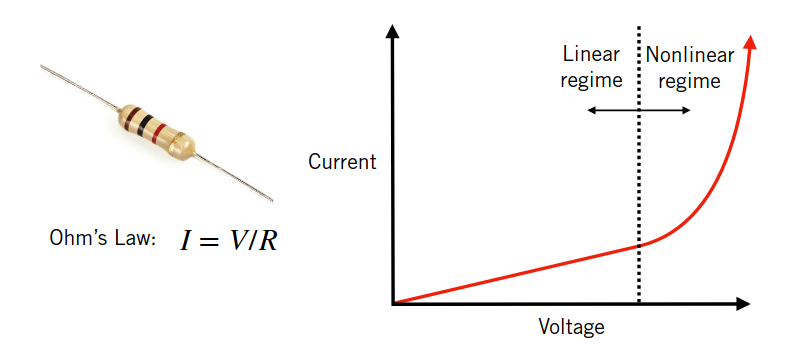
\includegraphics[width=0.8\textwidth]{chapters/chapter3/figures/resistor_curve.png}
%     \caption{Curva experimental de corrente vs tensão Resistor}
% \end{figure}

O método de linearização se da ao encontrar a função linear do sistema no ponto $\textcolor{red}{a}$ (Fig. \ref{fig:taylor}) através da Expansão da Série de Taylor, conforme demonstrado na figura \fig{fig:taylor}.

\begin{figure}
    \centering
    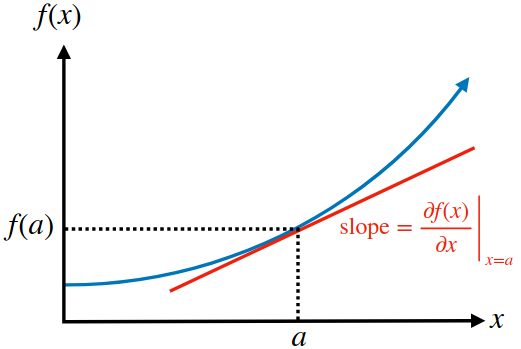
\includegraphics[width=0.8\textwidth]{chapters/chapter3/figures/taylor.pdf}
    \caption{Série de Taylor - Linearização}
    \label{fig:taylor}
\end{figure}

\begin{equation}
    \label{eq:taylor1}
    f(x,a) = \textcolor{red}{f(a) + \left. \frac{\partial f(x)}{\partial x} \right\vert_{x=a}(x-a)}
    \textcolor{gray}{+\frac{1}{2!}\left. \frac{\partial^2 f(x)}{\partial^2 x} \right\vert_{x=a}(x-a)^2 + \cdots}
\end{equation}

    Para o EKF, apenas a aproximação de primeira ordem é utilizada, conforme \eq{eq:taylor1} e \eq{eq:taylor2}.

\begin{equation}
    \label{eq:taylor2}
    \begin{split}
        g(u_t, x_{t-1}) \approx & g(u_t, \mu_{t-1}) + \frac{\partial g(u_t, \mu_{t-1}) }{\partial x_{t-1}}(x_{t-1}-\mu_{t-1}) \\
        g(u_t, x_{t-1}) \approx & g(u_t, \mu_{t-1}) + \color{red}{G_t}(x_{t-1}-\mu_{t-1})
    \end{split}
\end{equation}
onde $\color{red}G_t$ é calculado pela Matriz Jacobiana.

Bem como, para equação que representa a saída do sistema, temos \eq{eq:taylor4}.

\begin{equation}
    \label{eq:taylor4}
    \begin{split}
        h(x_t) \approx & h(\overline{\mu}_t) + \frac{\partial h(\overline{\mu}_t) }{\partial x_{t}}(x_{t}-\overline{\mu}_{t}) \\
        h(x_t) \approx & h(\overline{\mu}_t) + \color{blue}{H_t}(x_{t}-\overline{\mu}_{t})
    \end{split}
\end{equation}
onde $\color{blue}H_t$ é calculado pela Matriz Jacobiana.

A matriz Jacobiana demonstrada em $G_t$ e $H_t$ é expressa na forma generalizada pela \eq{eq:taylor5}.

\begin{equation}
    \label{eq:taylor5}
    \mathbb{J}
    =
    \frac{d \mathbf{f}}{d \mathbf{x}}
    =
    \left[ \frac{\partial \mathbf{f}}{\partial q_1}
        \cdots \frac{\partial \mathbf{f}}{\partial x_n} \right]
    =
    \begin{bmatrix}
        \frac{\partial f_1}{\partial x_1} & \cdots &
        \frac{\partial f_1}{\partial x_n}                   \\
        \vdots                            & \ddots & \vdots \\
        \frac{\partial f_m}{\partial x_1} & \cdots &
        \frac{\partial f_m}{\partial x_n}
    \end{bmatrix}
\end{equation}

Desta forma, pode-se reescrever o Algoritmo \ref{algo:kf} através da linearização do sistema pelo Algoritmo \ref{algo:ekf}.

\begin{algorithm}[H]
    \caption{Extended-Kalman-Filter}
    \begin{algorithmic}[1]
    \Procedure{Prediction}{$\mu_{t-1}, {\textstyle\sum}_{t-1}, u_t$}
        \State $\overline{\mu}_t = g(u_t, \mu_{t-1})$
        \State $ \overline{\textstyle\sum}_t = G_t {\textstyle\sum}_{t-1} G_t^T+ Q_t$ 
        \State \textbf{Return} $\left(\overline{\mu}_t, \overline{\textstyle\sum}_t\right)$
    \EndProcedure
    \Procedure{Update}{$\overline{\mu}_{t}, \overline{\textstyle\sum}_{t}, z_t$}
        \State $K_t = \overline{\textstyle\sum}_tH_t^T(H_t\overline{\textstyle\sum}_tH_t^T+R_t)^{-1}$
        \State $\mu_t  = \overline{\mu}_t + K_t(z_t -h(\overline\mu_t))$
        \State{$\textstyle\sum_t = (I-K_t H_t)\overline{\textstyle\sum}_t$}
        \State \textbf{Return} $\left(\mu_t, \textstyle\sum_t\right)$
    \EndProcedure
    \end{algorithmic}
    \label{algo:ekf}
\end{algorithm}


% \begin{frame}[c]{Extended Kalman Filter}
%     \framesubtitle{Exercício - Deslocamento Carro - Extended Kalman Filter}    \begin{columns}
%         \begin{column}[c]{0.4\textwidth}
%             \begin{figure}
%                 \centering
%                 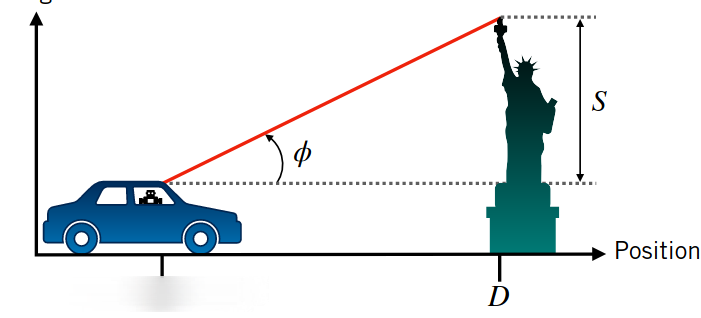
\includegraphics[width=1\textwidth]{./images/kalman_car2.png}
%                 \caption{Exemplo Deslocamento Carro}
%             \end{figure}
        
%         Tempo contínuo
%         \begin{equation*}
%            \left\{
%             \begin{matrix}
%                 s = & s_0 + vt \\
%                 v = & v_0 + at
%             \end{matrix}, 
%             \quad
%             \mathbf{x} = 
%             \begin{bmatrix}
%                 x \\
%                 \dot{x}
%             \end{bmatrix},
%             \right.
%         \end{equation*}
        
%         \begin{equation*}
%             \text{e, }\mathbf{u}=a
%         \end{equation*}

%         \end{column}
%         \begin{column}[c]{0.6\textwidth}
            
%             \textbf{Eq. Movimento - Tempo Discreto}:

%             \begin{equation*}
%                 \mathbf{x}_t = 
%                 \begin{bmatrix}
%                         1 & \Delta t \\
%                         0 & 1
%                 \end{bmatrix}
%                 \mathbf{x}_{t-1} +
%                 \begin{bmatrix}
%                         0 \\
%                         \Delta t
%                 \end{bmatrix}
%                 \mathbf{u}_{t-1} +
%                 \mathbf{w}_{t-1}
%             \end{equation*}

%             \textbf{Eq. Sensor - Tempo Discreto}:

%             \begin{equation*}
%                 \mathbf{z}_t = \phi_t  = 
%                 \tan^{-1}\left(\frac{S}{D-x_t} \right) +
%                 v_{t}
%             \end{equation*}            

%             \textbf{Ruído}:

%             $\mathbf{w}_t \sim \mathcal{N} 
%                 \left(
%                     \begin{bmatrix}
%                     0 \\ 0    
%                     \end{bmatrix},
%                     \begin{bmatrix}
%                     0.1 & 0 \\
%                     0   & 0.1
%                 \end{bmatrix}
%                 \right)$ e :
            
%             $ v_t \sim \mathcal{N} (0,0.05)$

%         \end{column}
%     \end{columns}
% \end{frame}



% \begin{frame}[c]{Extended Kalman Filter}
%     \framesubtitle{Exercício - Deslocamento Carro - Extended Kalman Filter}
    
%     \begin{itemize}
%         \item 1) Dado o sistema que descreve o deslocamento do carro acima,
%         calcule o primeiro passo do algoritmo Extended Kalman Filter.
%     \end{itemize}

%     \begin{columns}
%         \begin{column}[c]{0.4\textwidth}
%             \begin{figure}
%                 \centering
%                 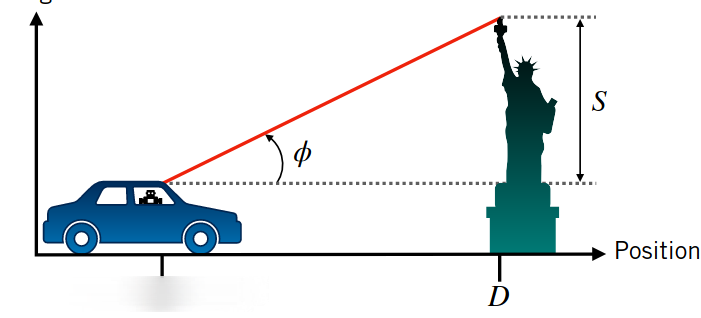
\includegraphics[width=1\textwidth]{./images/kalman_car2.png}
%                 \caption{Exemplo Deslocamento Carro}
%             \end{figure}
            
%         \end{column}
%         \begin{column}[c]{0.6\textwidth}
            
%             \textbf{Condições Iniciais}:

%             \begin{equation*}
%                 \mu_0 \sim \mathcal{N} \left( 
%                     \begin{bmatrix}
%                         0 \\ 5
%                     \end{bmatrix}, 
%                     \begin{bmatrix}
%                         0.01 & 0 \\
%                         0 & 1
%                     \end{bmatrix} \right)
%             \end{equation*}

%             $\Delta t = 0.5s$

%             $u_0 = -2m/s^2$

%            $z_1 = \frac{\pi}{6} rad$ 

%            $D = 40m$

%            $S = 20m$

%         \end{column}
%     \end{columns}
% \end{frame}




% \section{Glossary}
% \begin{Glossary}
% \item[360 Degree Review] Performance review that includes feedback from superiors, peers, subordinates, and clients.
% \item[Abnormal Variation] Changes in process performance that cannot be accounted for by typical day-to-day variation. Also referred to as
% non-random variation.
% \item[Acceptable Quality Level (AQL)] The minimum number of parts that must comply with quality standards, usually stated as a percentage.
% \item[Activity] The tasks performed to change inputs into outputs.
% \item[Adaptable] An adaptable process is designed to maintain effectiveness and efficiency as requirements change. The process is
% deemed adaptable when there is agreement among suppliers, owners, and customers that the process will meet
% requirements throughout the strategic period.
% \end{Glossary}



